\chapter{Types of NoSQL databases}
\noindent Structured Query Language, or SQL, was developed by IBM following \textcite{coddRelationalModelData1970}'s groundbreaking 
publication in the ACM journal, with the first commercial SQL implementation being published by Oracle in 1979 \autocite{oracleHistorySQL}.
SQL powers many relational database systems even today, though the problems associated with its age, most notably in 
the speed of its operations, are beginning to show in modern systems. Therefore, NoSQL ("Not Only SQL") was developed as 
an extension of SQL, allowing data to be stored in a non-tabular, non-relational format for efficient storage of
semi-structured and unstructured data in a flexible, functional and scalable model for faster operations than standard 
relational databases in most scenarios \autocite{googlecloudWhatNoSQLDatabases, awsWhatNoSQLDatabase}. There are a wide variety of NoSQL 
database types which vary in complexity, functionality and purpose, meaning that identification of the most suitable type is paramount 
for maximum efficiency. 

% TODO: Talk about ACID:
% ?     Atomicity - A statement is fully executed or not executed at all.
% ?     Consistency - Transactions only occur in predefined ways. (Helps prevent impacts of corruption)
% ?     Isolation - Concurrent transactions don't interfere with each other.
% ?     Durability - Changes are saved, even in the event of system failure. 
% *    https://www.databricks.com/glossary/acid-transactions

\section{Document database}\label{sec:DocDBs}
% ? MongoDB is a document database.
% * General purpose databases.
Document databases are intuitive, flexible and horizontally scalable databases that work well in a wide variety of use cases
for both transactional and analytical purposes, including IoT data and real-time analytics \autocite{mongodbDocumentDatabaseNoSQL}.
They store records as "documents", which store an object's data and metadata, in a format such as JSON, BSON, or XML\footnote{JavaScript Object Notation, Binary JSON and Extensible Markup Language, respectively.}. Details and examples of these file types can be found in Appendix A.

% TODO: Finish Appendix A, where you talk about and give examples of each of these. See Lab 4 slides for modelling relationships with JSON.

\begin{figure}[H]
    \centering
    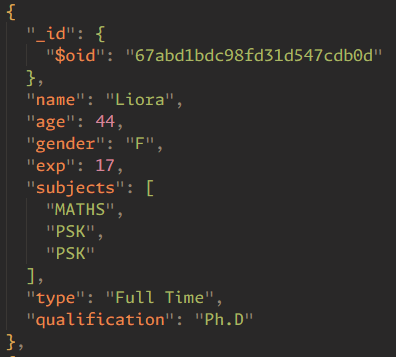
\includegraphics[width=0.7\textwidth]{NoSQL DBs/Doc/ExampleDoc}
    \caption{An example of a JSON Document.\label{fig:ExampleDoc}}
\end{figure}

\noindent Figure \ref{fig:ExampleDoc} depicts an example JSON document in MongoDB\footnote{MongoDB actually stores data as BSON, though it translates between the two when queried.}, a popular DBMS
for document databases. It contains the data of a singular example school teacher, storing details such as their name, age and subject expertise, as well as a unique internal object ID used by MongoDB to identify that document. The data itself is of varying types including 
strings, integers and arrays, which makes document databases easily integrable into a development workflow due to the direct 
storage of object types used in programming languages like Python and JavaScript.

% TODO: Has enough been written here?

\para Popular services for document databases include Databricks \autocite{databricksDataAICompany2023} Couchbase \autocite{couchbaseCouchbaseBestFree}, and the previously mentioned MongoDB \autocite{mongodbDocumentDatabaseNoSQL}.


\section{Key-value database}
% ? Redis is a key-value database.
% ! While that's true, it's also an in-memory database.
% * Very fast, very simple.
Key-value databases are primarily reputed for their speed and simplicity, functioning by storing each record as a key-value pair.
Rather than having to search through massive amounts of irrelevant data for a query, key-value databases can instead search 
through their stored keys to retrieve results within milliseconds or even microseconds if used in-memory \autocite{redisRedisFAQ}.
While this is excellent for simple queries to retrieve specific known records, this same property also causes major limitations in
that retrieving data based on values, such as finding all users over a given age, would require the entire database to be searched,
making key-value databases best suited for real-time data access and caching where simpler queries are used \autocite{mongodbWhatKeyValueDatabase}.

% TODO: You've spoke of key-value negatives here, so go back and do it for documents too.
% TODO: Some kind of image for key-value sample data.
% TODO: What's the difference between key-value and document?

\para Notable software options used across industry for key-value databases include Amazon's DynamoDB \autocite{awsFastNoSQLKeyValue} and Redis \autocite{redisWhatKeyValueDatabase}. 


\section{Column-oriented database}
% * Stores data in columns rather than rows.
% * Fast reading, slow writing. 
% * Better for OLAP than OLTP iirc.
% ! In the scenario, the slow writing means it's unwanted. Client wants IoT sensor data recorded, so it'll be lots of writing.
% ? Also known as wide-column stores, which may be the preferred term for the module spec.


\section{Graph database}
% ? Neo4J is a graph database.